\newpage
\section{Ammonia Adsorption/Desorption Process Dynamics}

\begin{figure}[H]
    \centering
    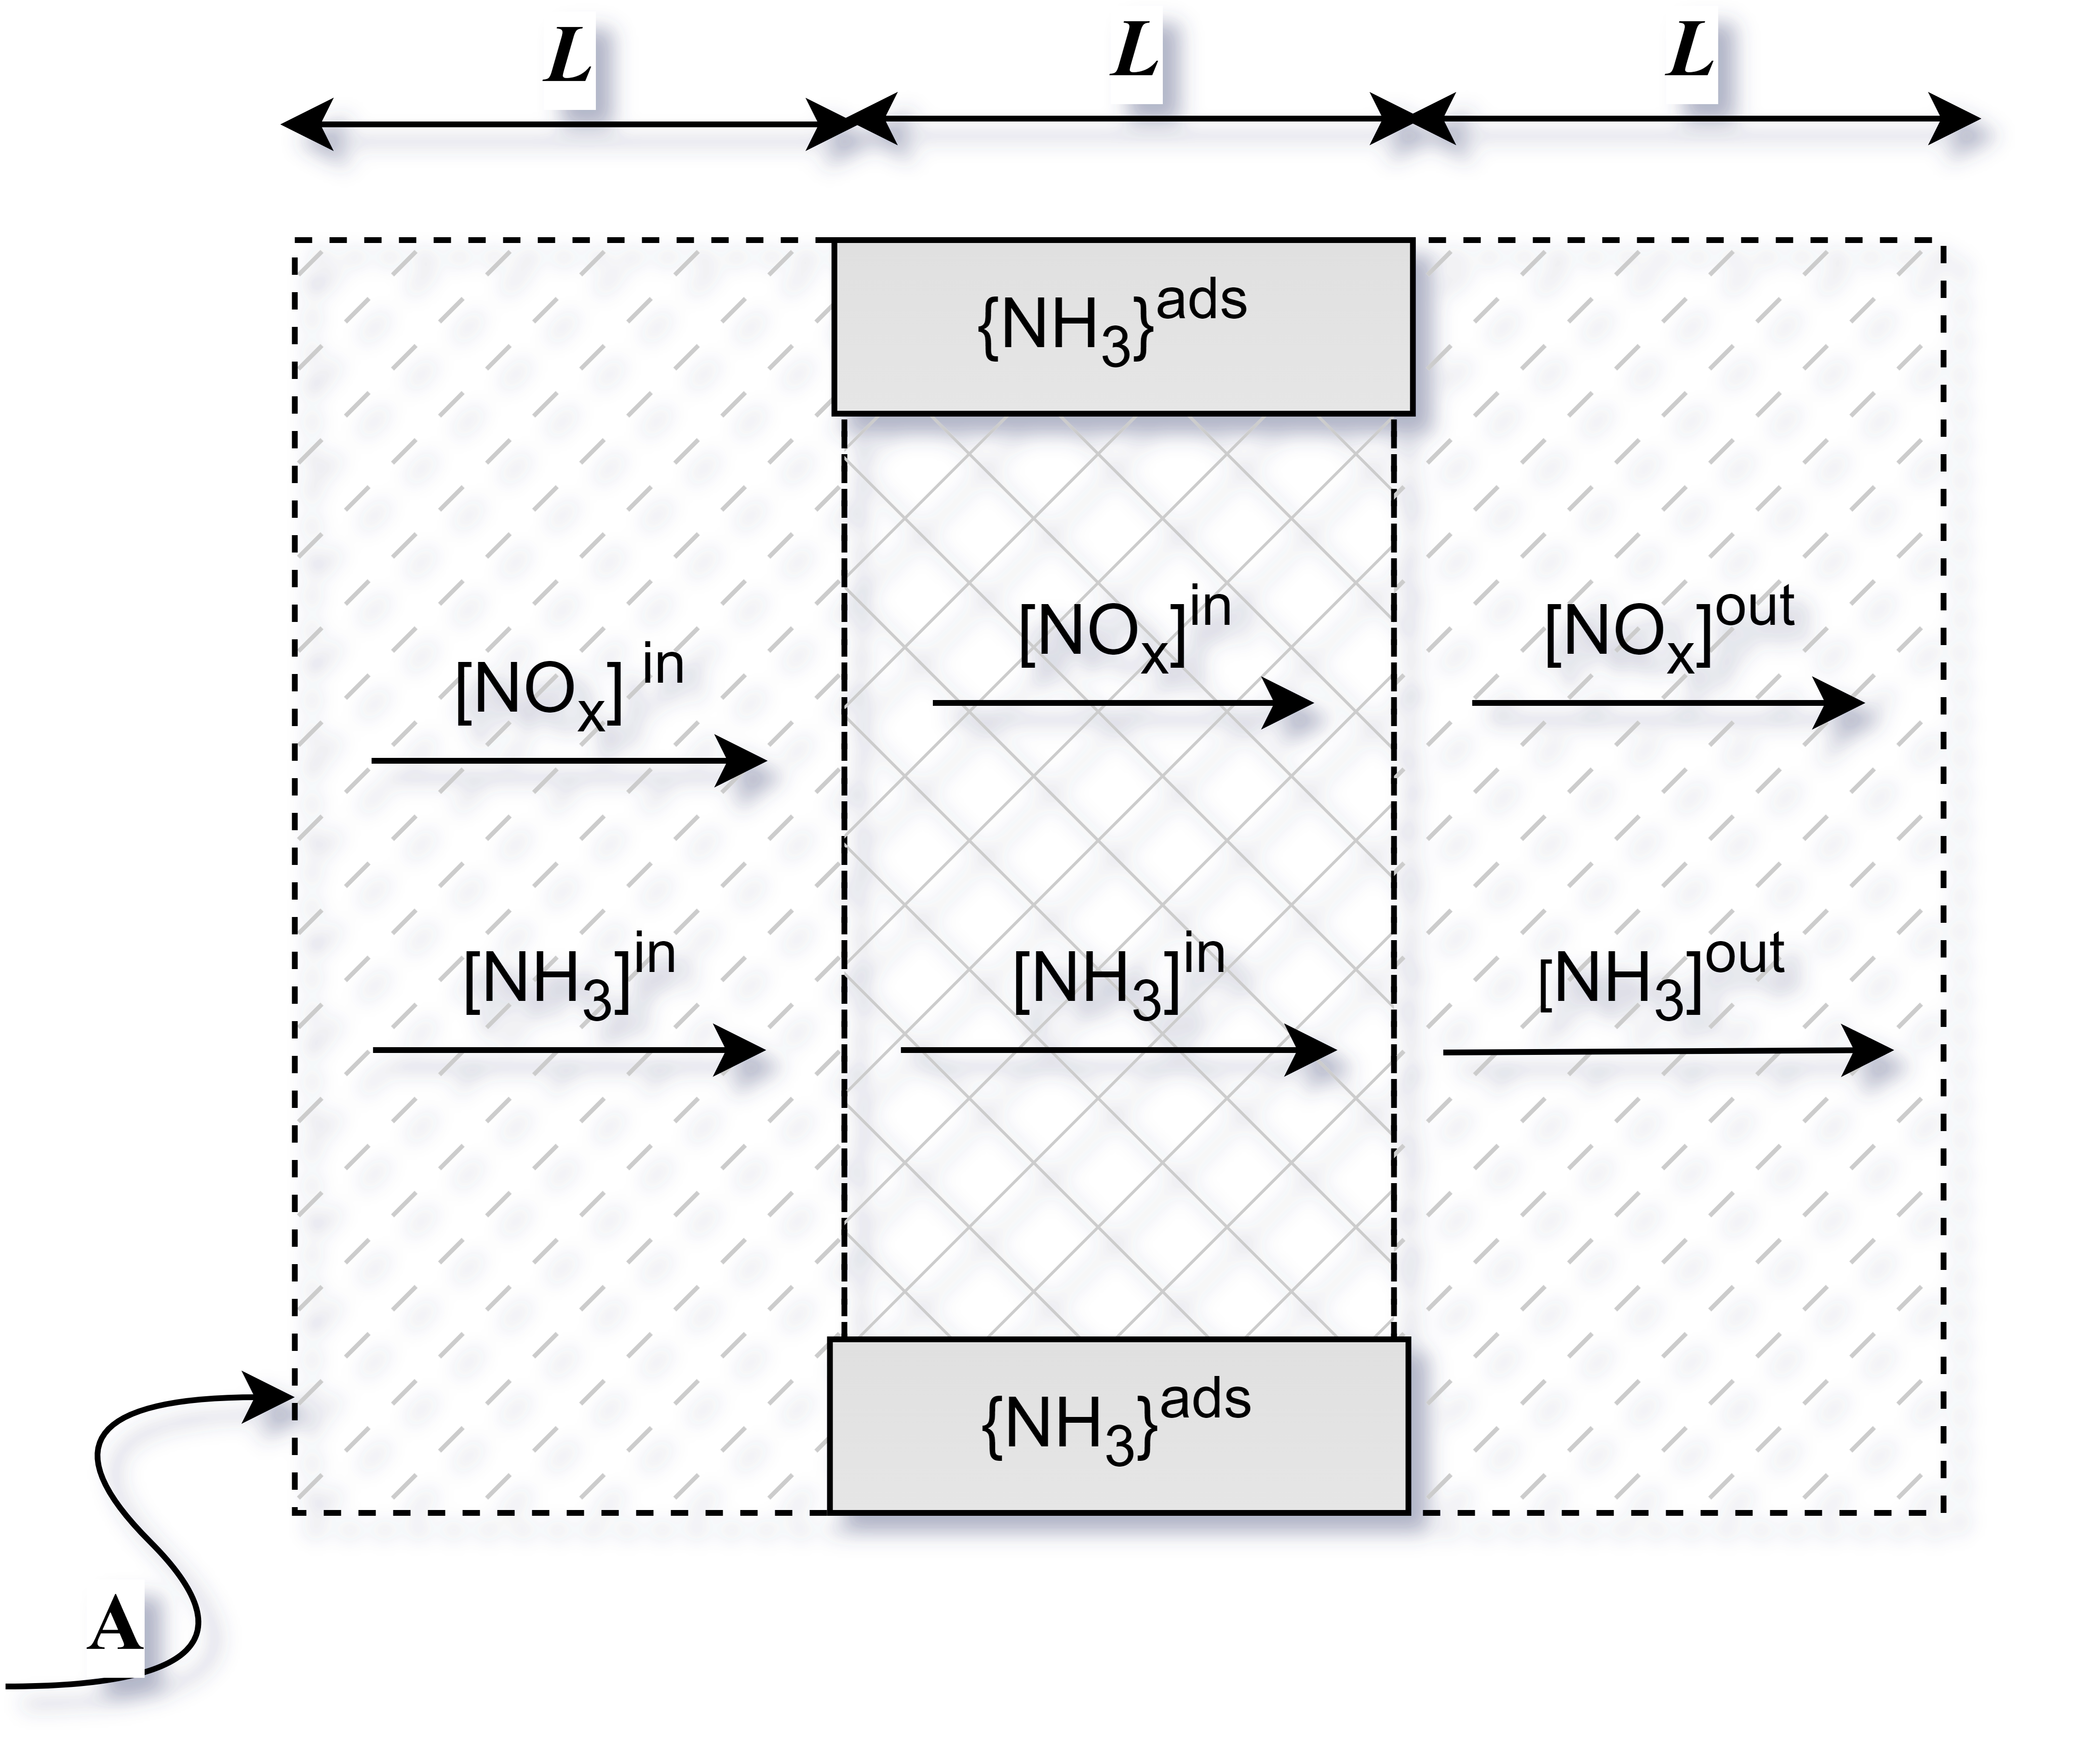
\includegraphics[width=0.5\textwidth]{./figs/scr_sys/plug_flow_discrete.png}
    \caption{Discrete plug-flow reactor model}
    \label{fig:plug_flow_discrete}
\end{figure}


The ammonia adsorption/desorption process dynamics involve all the three
above-mentioned reactions. The gaseous ammonia that enters the catalyst chamber
gets adsorbed on the to free sites on the catalyst surface at a rate
promotional to the volumetric concentration of the gaseous ammonia and the
surface concentration of the free sites. The adsorbed ammonia then either reacts
with the gaseous $NO_x$ (Eiley-Rideal Mechanism) releasing $N_2$ and $H_2O$ or
decomposes to form $N_2$ and $H_2O$ (Surface Decomposition). In either
case, the process frees up the adsorption sites for the next cycle of gasueous ammonia.

\begin{align}
    4 NH_3 ^{ads} + 4 NO + O_2 &\xrightarrow[]{k_{scr}} 4 N_2 + 6 H_2O \\
    4 NH_3^{ads} + 3 O_2 &\xrightarrow[]{k_{oxi}} 2 N_2 + 6 H_2O \\
    NH_3 + \Theta_{free} &\xrightleftharpoons[k_{des}]{k_{ads}} NH_3^{ads}
\end{align}


Thus, the rate of ammonia adsorption on the catalyst surface can be modeled as:

\begin{align}
    \frac{d \con{NH_3}^{ads}}{dt} &= r_{ads} - r_{des} - r_{scr} - r_{oxi}\\
    r_{ads} &= k_{ads} \con{NH_3}^{in} \lr{\Gamma - \con{NH_3}^{ads}}\\
    r_{des} &= k_{des} \con{NH_3}^{ads}\\
    r_{scr} &= k_{scr} \con{NH_3}^{ads} \con{NO_x}^{in}\\
    r_{oxi} &= k_{oxi} \con{NH_3}^{ads}
\end{align}

\itbf{Note:} $\Gamma$ and $\con{NH_3}^{ads}$ are surface concentrations (in
$moles/cm^2$) while the rest are volumetric concentrations (in $moles/cm^3$).
The rate constant units are adjusted appropriately to make the rate equations consistent.

The units of all the rates and rate constants are tabulated bellow:

\begin{align*}
    r_{ads} &= \frac{moles}{cm^2 \cdot s} &
    k_{ads} &= \frac{cm^3}{moles \cdot s} \\
    r_{des} &= \frac{moles}{cm^2 \cdot s} &
    k_{des} &= s^{-1} \\
    r_{scr} &= \frac{moles}{cm^2 \cdot s} &
    k_{scr} &= \frac{cm^3}{moles \cdot s} \\
    r_{oxi} &= \frac{moles}{cm^2 \cdot s} &
    k_{oxi} &= s^{-1}
\end{align*}


\itbf{Note:}In this section we are interested in the Surface rates where the
products are assumed to linger just on the surface of the catalyst. The surface
rates of the gaseous products/reactants are can be converted to volumetric
rates by using the convention factor $A_{scr}/V$ where $A_{scr}$ is the area of
the SCR catalyst and V is the volume of the catalyst chamber. This assumes that
there is instantaneous mixing of the close to  surface moles with the gaseous
moles. Thus,
\begin{align}
    k^{vol} = \underbrace{\lr{\frac{A_{scr}}{V}}}_{k_{s2v} \, (cm^{-1})} k^{surf}
\end{align}

% ==============================================================================

\subsection{Molar conservation at the scale of residence time}

The molar storage on the catalyst surface changes at the end of every residence
time and a "fresh" set of gaseous reactants enters the catalyst chamber. And,
with in the sample time, the volumetric concentrations of the gaseous reactants
can be considered constant. \itbf{Let there be $n$ residence times within one
sample time.} Then, the molar conservation for the adsorption/desorption process
can be written as:

\begin{align*}
    \mol{NH_3}^{ads} (k + \tau) &= \mol{NH_3}^{ads} (k) + A_{scr} \int_{0}^{\tau} \dot{\con{NH_3}}^{ads} (k) dt\\
    \mol{NH_3}^{ads} (k + 2\tau) &= \mol{NH_3}^{ads} (k + \tau) + A_{scr} \int_{0}^{\tau} \dot{\con{NH_3}}^{ads} (k + \tau) dt\\
    \vdots&\\
    \mol{NH_3}^{ads} (k + n\tau) &= \mol{NH_3}^{ads} (k + (n-1)\tau) + A_{scr} \int_{0}^{\tau} \dot{\con{NH_3}}^{ads} (k + (n-1)\tau) dt
\end{align*}

\begin{align}
    \mol{NH_3}^{ads}(k + 1) = \mol{NH_3}^{ads} (k + n\tau) &= \mol{NH_3}^{ads} (k) + A_{scr} \sum_{i=0}^{n-1} \int_{0}^{\tau} \dot{\con{NH_3}}^{ads} (k + i\tau) dt
\end{align}

Writing above equation interns of surface concentrations:
\begin{align}
    \con{NH_3}^{ads}(k + 1) = \con{NH_3}^{ads} (k + n\tau) &= \con{NH_3}^{ads} (k) + \underbrace{\sum_{i=0}^{n-1} \int_{0}^{\tau} \dot{\con{NH_3}}^{ads} (k + i\tau)}_{\Omega(k)}   dt
\end{align}
